%
% additional usepackage{beamerthemeshadow} is used
%  
%  \beamersetuncovermixins{\opaqueness<1>{25}}{\opaqueness<2->{15}}
%  with this the elements which were coming soon were only hinted
\documentclass[xcolor=dvipsnames]{beamer}
\usepackage{beamerthemeshadow}
\usepackage[ngerman]{babel}
%\usetheme{Copenhagen}
\usetheme{CambridgeUS}

\usecolortheme[named=BrickRed]{structure}
\useinnertheme{rounded}
\setbeamercovered{transparent}

\begin{document}
\title{Regulated Array Grammars of Finite Index}  
\author{C. Gruber, J. Reiter}
\institute{TU Wien}
%\date{\today} 
\date{3.M\"arz, 2010}

\frame{\titlepage} 

\frame{\frametitle{Table of contents}\tableofcontents} 


\section{Preliminaries} 
\subsection{n-dimensional array}
\frame{\frametitle{n-dimensional array} 
Ein n-dimensionales Array $A$  \"uber ein Alphabet $V$ (Menge aller non-terminal und terminal Symbole) ist eine Funktion 

\begin{eqnarray*}
A : Z^n \rightarrow V \cup \{\#\} & n \in N = \{1,2,...\}
\end{eqnarray*}

wobei 
\[ shape(A) = \{ v \in Z^n | A(v) \not = \# \}
\]
endlich ist und $\# \not \in  V$ als \textit{background} oder \textit{blank Symbol} bezeichnet wird. Das Array $A$ kann nun so definiert werden
\[ A = \{ (v,A(v)) \ | \ v \in shape(A) \}.
\]
}

\frame{\frametitle{n-dimensional array production and grammar} 
Eine n-dimensionale Array Produktion $p$ \"uber dem Alphabet $V$ ist ein Tripel $(W,A_1,A_2)$ wobei $W \subseteq Z^n$ eine endliche Menge von Koordinaten ist und $A_1$ und $A_2$ Abbildungen von $W$ auf $V \cup \{\#\}$ sind.
\newline
\newline
Eine n-dimensionale Array Grammatik kann nun als Sechstupel 
\[ G = (n,V_N,V_T,\#,P,\{(v_0,S)\})
\]
definiert werden. $\{(v_0,S)\}$ wird als Startarray (Axiom), $v_0$ als Startvektor und $S$ als das Startsymbol bezeichnet.
}

\section{Control mechanisms} 
\frame{\frametitle{matrix grammar} 
Eine Matrixgrammatik $G_M$ ist ein 4-Tupel

\[ G_M = (V_N,V_T,(M,F),S),
\]
$F$ kann auch als Fehlermenge bezeichnet werden. Ist $F= \emptyset$, dann kann $G_M$ als Matrixgrammatik ohne appearence checking bezeichnet werden.
}

\frame{\frametitle{graph controlled grammar} 
Eine graph-controlled Grammatik $G_P$ ist ein 4-Tupel

\[ G_M = (V_N,V_T,(R,L_{in},L_{fin}),S),
\]
$R$ ist eine endliche Menge von Regeln $r$ der Form 
\[ (l(r) : p(l(r)), \sigma (l(r)), \varphi (l(r))).
\]
Falls alle Felder $\varphi (l(r))$ leer sind f\"{u}r alle $r \in R$, dann kann $G_P$ als graph-controlled Grammatik ohne appearence checking bezeichnet werden.

\pause

\begin{alertblock}{}
Matrix- und graph-controlled Grammatiken k�nnen in Arraygrammatiken direkt \"{u}bergef\"{u}hrt werden, indem ihre Produktionen durch Arrayproduktionen ersetzt werden.
\end{alertblock}
}

\frame{\frametitle{bounded derivations} 
\begin{alertblock}{Index einer Ableitung}
Der Index einer Ableitung $D$ eines Terminalobjekts $w$ in einer Grammatik $G$ ist mit der maximalen Anzahl von non-terminal Symbolen, die in einem Zwischenableitungsschritt vorkommen, definiert und wird mit $ind_{G,D}(w)$ bezeichnet.
\end{alertblock}

\pause

Weiters bezeichnet $ind_{G,min}(w)$ bzw. $ind_{G,max}(w)$ das Minimum bzw. das Maximum aus der Menge

\[ \{ind_{G,D}(w) \ | \ w \ \mathrm{is \ generated \ by} \ G \}
\]
Entsprechend gibt es nun die Definition f\"{u}r die Grammatik
\begin{eqnarray*}
ind_{Y}(G) = sup \{ind_{G,Y}(w)\ | \ w \ \mathrm{is \ generated \ by} \ G \} & Y \in \{min,max\}
\end{eqnarray*}
Bei einer endlichen Index Restriktion nur Objekte $w$, die von einer Grammatik $G$ mit einer Ableitung $ind_{G,Y}(w) \leq k$ f\"{u}r $Y \in \{min,max\}$.
}

\frame{\frametitle{grammar with prescribed teams}
Eine Grammatik mit prescribed teams $G_t$ ist ein 4-Tupel

\[ G_t = (V_N,V_T,(P,R,F),S),
\]
$G = (V_N,V_T,P,S)$ ist eine kontextfreie Grammatik, $R$ ist eine endliche Menge von Teams aus $P$ und $F$ ist die Menge von Produktionen, die bei dem appearence checking \"{u}bersprungen werden k�nnen. Ist $F= \emptyset$, dann kann $G_t$ als Grammatik mit prescribed teams ohne appearence checking bezeichnet werden.
}

\frame{\frametitle{Beispiel f\"{u}r eine Grammatik mit prescribed teams (1)}
\textbf{2-dimensionale Array-Grammatik mit prescibed teams:}

\[ G=(n,\left\{ D,E,L,Q,R,S,U \right\} , \left\{ a \right\} , \# , (P,R,F), \left\{ ((0,0),S) \right\} )
\]

\[P= \left\{
\begin{array}{l}
	\# \\
	S \#
\end{array}
\rightarrow
\begin{array}{l}
	L \\
	a D
\end{array}
,
\begin{array}{l}
	\# \\
	L 
\end{array}
\rightarrow
\begin{array}{l}
	L \\
	a 
\end{array}
,
\begin{array}{l}
	D \# \\
\end{array}
\rightarrow
\begin{array}{l}
	a D \\
\end{array} 
,
\begin{array}{l}
	\# \# \\
	L &
\end{array}
\rightarrow
\begin{array}{l}
	a U \\
	a
\end{array}
,\right \]
\[
\begin{array}{l}
	D \# \\
\end{array}
\rightarrow
\begin{array}{l}
	a R \\
\end{array}
,
\begin{array}{l}
 \# \\
 R
\end{array}
\rightarrow
\begin{array}{l}
	R \\
	a
\end{array}
,
\begin{array}{l}
	U \# \\
\end{array}
\rightarrow
\begin{array}{l}
	a U \\
\end{array}
,\ \ \ \ \ \ \ \ \ \ \ 
\]
\[
\left
\begin{array}{l}
	U \# \\
\end{array}
\rightarrow
\begin{array}{l}
	a U \\
\end{array}
,
	U \rightarrow E,
\begin{array}{l}
\# \\
	R
\end{array}
\rightarrow
\begin{array}{l}
Q \\
a
\end{array}
,
R \rightarrow a,
E \rightarrow a
\right\} 
\]
}

\frame{\frametitle{Beispiel f\"{u}r eine Grammatik mit prescribed teams (2)}
\[R= \left\{
\left\langle 
\begin{array}{l}
	\# \\
	S \#
\end{array}
\rightarrow
\begin{array}{l}
	L \\
	a D
\end{array} \right\rangle
,
\left\langle  \begin{array}{l}
	\# \\
	L 
\end{array}
\rightarrow
\begin{array}{l}
	L \\
	a 
\end{array}
,
\begin{array}{l}
	D \# \\
\end{array}
\rightarrow
\begin{array}{l}
	a D \\
\end{array} \right\rangle \right 
,\]
\[ \left\langle 
\begin{array}{l}
	\# \# \\
	L &
\end{array}
\rightarrow
\begin{array}{l}
	a U \\
	a
\end{array}
,
\begin{array}{l}
	D \# \\
\end{array}
\rightarrow
\begin{array}{l}
	a R \\
\end{array} \right\rangle
,
\left\langle 
\begin{array}{l}
 \# \\
 R
\end{array}
\rightarrow
\begin{array}{l}
	R \\
	a
\end{array}
,
\begin{array}{l}
	U \# \\
\end{array}
\rightarrow
\begin{array}{l}
	a U \\
\end{array} \right\rangle
,\ \ \ \ \ \ \ \ 
\]
\[\ \ \ \ \ \ \ \ \ \ 
\left
\left\langle 
\begin{array}{l}
	U \# \\
\end{array}
\rightarrow
\begin{array}{l}
	a U \\
\end{array}
,
	U \rightarrow E,
\begin{array}{l}
\# \\
	R
\end{array}
\rightarrow
\begin{array}{l}
Q \\
a
\end{array} \right\rangle
,
\left\langle 
R \rightarrow a,
E \rightarrow a
\right\rangle
\right\} 
\]
\newline
\[
F= \left\{	
\begin{array}{l}
\# \\
	R
\end{array}
\rightarrow
\begin{array}{l}
Q \\
a
\end{array} \right\}
\]

Ableitungssequenz:
\[
	S \Rightarrow_G 
\begin{array}{l}
	L \\
	a\ D
\end{array}
\Rightarrow_G 
\begin{array}{l}
a\ U \\
a \\
a\ a\ R
\end{array}
\Rightarrow_G
\begin{array}{l}
a\ a\ U \\
a \\
a\ a\ R
\end{array}
\Rightarrow_G
\begin{array}{l}
a\ a\ E \\
a\ \ \ R \\
a\ a\ a
\end{array}
\Rightarrow_G
\begin{array}{l}
a\ a\ a\ \\
a\ \ \ a \\
a\ a\ a\ 
\end{array}\]

}

\section{The finite index restriction} 
\frame{\frametitle{Gefolgerte Resultate} 
\begin{alertblock}{Theorem 1}
F\"{u}r jedes $k \in \{fin\} \cup \{j \ | \ j\geq 1 \}$, gilt
\[PT^{\left\lceil k \right\rceil}(cf) = PT_{ac}^{\left\lceil k \right\rceil}(cf) = Z^{Y, \left\lceil k \right\rceil}(cf) = Z^{min, \cap\left\lceil k \right\rceil}(cf)
\]
f\"{u}r alle $Z \in \{M,M_{ac},P,P_{ut},P_{ac}\}$ und $Y \in \{min,max\}$.
\end{alertblock}

\pause

\begin{alertblock}{Theorem 2}
F\"{u}r $X \in \{n-\#-cf, n-cf \ | \ n \geq 1\}$, gilt

\begin{enumerate}
\item $PT^{\left\lceil fin \right\rceil}(X) = Z^{Y, \left\lceil fin \right\rceil}(X) = Z^{min, \cap \left\lceil fin \right\rceil}(X)$ und auch
\item $PT_{ac}^{\left\lceil fin \right\rceil}(X) = Z_{ac}^{Y, \left\lceil fin \right\rceil}(X) = Z_{ac}^{min, \cap \left\lceil fin \right\rceil}(X)$
\end{enumerate}

f\"{u}r alle $Z \in \{M,P\}$ und $Y \in \{min,max\}$.
\end{alertblock}
}

\frame{\frametitle{Gefolgerte Resultate (2)}
\begin{alertblock}{Theorem 3}
	F\"{u}r alle $k\in \left\{ fin\right\} \cup \left\{ j | j \geq 1 \right\}$ gilt
\begin{enumerate}
	\item $PT^{\left\lceil k \right\rceil} (X) = Z^{Y,\left\lceil k \right\rceil} (X) = Z^{min,\cap \left\lceil k \right\rceil} (X)\ genau\ so\ wie$
	\item $PT_{ac}^{\left\lceil k \right\rceil} (X) = Z_{ac}^{Y,\left\lceil k \right\rceil} (X) = Z_{ac}^{min,\cap \left\lceil k \right\rceil} (X)$
\end{enumerate}
F\"{u}r alle $X\in \left\{ n-scf,n-scf_1 | n \geq 1\right\},\ Z\in \left\{ M,P\right\},\ und\ Y\in \left\{ min,max\right\}$.
\end{alertblock}

\begin{alertblock}{Theorem 4}
	F\"{u}r alle $X\in \left\{ 1-cf_1, 1-scf_1\right\}$ gilt
\[PT^{\left\lceil  1\right\rceil} (X) = PT_{ac}^{\left\lceil  1\right\rceil} (X) = Z^{Y,\left\lceil 1 \right\rceil} (X) = Z^{min,\cap \left\lceil 1 \right\rceil} (X) = L(1-reg)\]

F\"{u}r alle $Z\in \left\{ M,M_{ac},P,P_{ut},P_{ac}\right\}\ und\ Y\in \left\{ min,max\right\}$.
\end{alertblock}
}

\frame{\frametitle{Gefolgerte Resultate (3)}

\begin{alertblock}{Theorem 5}
	F\"{u}r alle $X\in \left\{ 1-cf_1, 1-scf_1\right\}\ und\ alle\ k\geq 2$ gilt
\[PT^{\left\lceil  k\right\rceil} (X) = PT_{ac}^{\left\lceil  k\right\rceil} (X) = Z^{Y,\left\lceil k \right\rceil} (X) = Z^{min,\cap \left\lceil k \right\rceil} (X) = PT^{\left\lceil  2\right\rceil} (X)\]\\
F\"{u}r alle $Z\in \left\{ M,M_{ac},P,P_{ut},P_{ac}\right\}\ und\ Y\in \left\{ min,max\right\}$.
$PT^{\left\lceil  2\right\rceil} (X)$ repr�sentiert eine Familie von String-Sprachen $L(lin)$.
\end{alertblock}
}

\section{Syntaktisches Pattern Recognition} 
\subsection{Aspekte der syntaktischen Character Recognition}
\frame{\frametitle{Stufen in Character Recognition} 

\begin{columns}
\begin{column}{7cm}
\begin{enumerate}
\item Anlegen von Daten
\item Preprocessing
\begin{itemize}
	\item Normalisierung und Rauscheliminierung: anschlie�end abbilden auf eine 20 x 25 Gitter
	\item Ausd�nnung (Skelletierung)
\end{itemize}
\item Syntaktische Analyse
\end{enumerate}
\end{column}
\begin{column}{5cm}

\begin{figure}	
	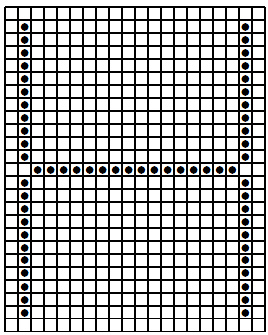
\includegraphics[width=0.70\textwidth]{character_H}
	\label{fig:character_H}
\end{figure}

\end{column}
\end{columns}
}

\frame{\frametitle{Beispiel zur Erkennung eines H}
\textbf{2-dimensionale Array-Grammatik mit prescibed teams:}

\[ G=(n,\left\{ S,L,R,D_L,U_L,D_R,U_R \right\} , \left\{ a \right\} , \# , (P,R,\emptyset ), \left\{ ((0,0),S) \right\} )
\]

\[P= \left\{
\begin{array}{l}
	S \#
\end{array}
\rightarrow
\begin{array}{l}
	LR \\
\end{array}
,
\begin{array}{l}
	\# L \\
\end{array}
\rightarrow
\begin{array}{l}
	L a\\ 
\end{array}
,
\begin{array}{l}
	R \# \\
\end{array}
\rightarrow
\begin{array}{l}
	a R \\
\end{array} 
,
\begin{array}{l}
	\# \\
	\ \ \ L \\
	\#
\end{array}
\rightarrow
\begin{array}{l}
	U_L \\
	\ \ \ a \\
	D_L
\end{array}
,\right \]
\[\ \ \ \ \ \ \ \ \ \ 
\begin{array}{l}
	\ \ \ \# \\
	R \\
	\ \ \ \#
\end{array}
\rightarrow
\begin{array}{l}
	\ \ \ U_R \\
	a \\
	\ \ \ D_R
\end{array}
,
\begin{array}{l}
	\# \\
	U_L
\end{array}
\rightarrow
\begin{array}{l}
	U_L \\
	a
\end{array}
,
\begin{array}{l}
	\# \\
	U_R
\end{array}
\rightarrow
\begin{array}{l}
	U_R \\
	a
\end{array}
,
\begin{array}{l}
	D_L \\
	\#
\end{array}
\rightarrow
\begin{array}{l}
	a \\
	D_L
\end{array}
,
\]
\[
\left
\begin{array}{l}
	D_R \\
	\#
\end{array}
\rightarrow
\begin{array}{l}
	a \\
	D_R
\end{array}
,
	U_L \rightarrow a,
	U_R \rightarrow a,
	D_L \rightarrow a,
	D_R \rightarrow a
\right\} \ \ \ \ \ \ \  
\]
}

\frame{\frametitle{Beispiel zur Erkennung eines H (2)}
\[R= \left\{
\left\langle 
\begin{array}{l}
	S \#
\end{array}
\rightarrow
\begin{array}{l}
	LR \\
\end{array} \right\rangle
,
\left\langle  \begin{array}{l}
	\# L \\
\end{array}
\rightarrow
\begin{array}{l}
	L a\\ 
\end{array}
,
\begin{array}{l}
	R \# \\
\end{array}
\rightarrow
\begin{array}{l}
	a R \\
\end{array}  \right\rangle \right 
,\ \ \ \ \ \ \ \ \ \ 
\]
\[ \left\langle 
\begin{array}{l}
	\# \\
	\ \ \ L \\
	\#
\end{array}
\rightarrow
\begin{array}{l}
	U_L \\
	\ \ \ a \\
	D_L
\end{array},
\begin{array}{l}
	\ \ \ \# \\
	R \\
	\ \ \ \#
\end{array}
\rightarrow
\begin{array}{l}
	\ \ \ U_R \\
	a \\
	\ \ \ D_R
\end{array} 
\right\rangle 
,\ \ \ \ \ \ \ \ \ \ \ \ \ \ \ \ \ 
\]
\[\ \ \ \ \ \ \ \ \ \ \ \ \ \ \ \ \ \ \ \ \ 
\left\langle 
\begin{array}{l}
	\# \\
	U_L
\end{array}
\rightarrow
\begin{array}{l}
	U_L \\
	a
\end{array}
,
\begin{array}{l}
	\# \\
	U_R
\end{array}
\rightarrow
\begin{array}{l}
	U_R \\
	a
\end{array}
,
\begin{array}{l}
	D_L \\
	\#
\end{array}
\rightarrow
\begin{array}{l}
	a \\
	D_L
\end{array} 
,
\begin{array}{l}
	D_R \\
	\#
\end{array}
\rightarrow
\begin{array}{l}
	a \\
	D_R
\end{array}
\right\rangle
,\ \ \ \ \ \ \ \ 
\]
\[\ \ \ \ \ \ \ \ \ \ 
\left
\left\langle 
	U_L \rightarrow a,
	U_R \rightarrow a,
	D_L \rightarrow a,
	D_R \rightarrow a
\right\rangle
\right\} \ \ \ \ \ \ \ \ \ \ \ \ \ \ \ \ \ \ \ \ \ \ \ \ \ \ 
\]
\newline

}

\frame{\frametitle{Beispiel zur Erkennung eines H (3)}
Ableitungssequenz:
\[
	S \Rightarrow_G 
\begin{array}{l}
	L\ R\\
\end{array}
\Rightarrow_G 
\begin{array}{l}
L\ a\ a\ R \\
\end{array}
\Rightarrow_G
\begin{array}{l}
U_L\ \ \ \ \ \ \ \ \ U_R \\
\ \ \ a\ a\ a\ a\ \  \\
D_L\ \ \ \ \ \ \ \ \ D_R
\end{array}
\Rightarrow_G
\begin{array}{l}
U_L\ \ \ \ \ \ \ \ \ U_R \\
a\ \ \ \ \ \ \ \ \ \ \ a \\
\ \ \ a\ a\ a\ a\ \  \\
a\ \ \ \ \ \ \ \ \ \ \ a \\
D_L\ \ \ \ \ \ \ \ \ D_R\end{array}
\Rightarrow_G
\]
\[
\begin{array}{l}
U_L\ \ \ \ \ \ \ \ \ U_R \\
a\ \ \ \ \ \ \ \ \ \ \ a \\
a\ \ \ \ \ \ \ \ \ \ \ a \\
\ \ \ a\ a\ a\ a\ \  \\
a\ \ \ \ \ \ \ \ \ \ \ a \\
a\ \ \ \ \ \ \ \ \ \ \ a \\
D_L\ \ \ \ \ \ \ \ \ D_R
\end{array}
\Rightarrow_G
\begin{array}{l}
a\ \ \ \ \ \ \ \ \ \ \ a \\
a\ \ \ \ \ \ \ \ \ \ \ a \\
a\ \ \ \ \ \ \ \ \ \ \ a \\
\ \ \ a\ a\ a\ a\ \  \\
a\ \ \ \ \ \ \ \ \ \ \ a \\
a\ \ \ \ \ \ \ \ \ \ \ a \\
a\ \ \ \ \ \ \ \ \ \ \ a \\
\end{array}
\]
}

\frame{\frametitle{M�gliche Probleme} 

\begin{columns}
\begin{column}{7cm}



\end{column}
\begin{column}{5cm}

\begin{figure}	
	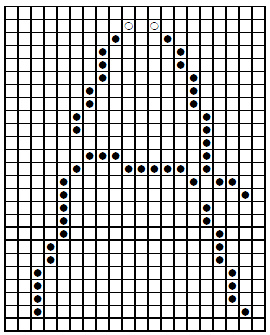
\includegraphics[width=0.80\textwidth]{bad_character_H}
	\label{fig:character_H}
\end{figure}

\end{column}
\end{columns}

}


\end{document}